\section{Results}

\subsection{Optimization method comparison}

Three optimization strategies were tested:

\begin{enumerate}
    \item \textbf{Brute-force}: All three waveplates are sequentially set to every possible position (0--154) and the power is measured at each point. This guarantees finding the global minimum but is extremely time-consuming.

    \item \textbf{Model-based fitting}: Multiple data points are collected and a $\sin$-curve is fitted to predict the minimum position. This assumes the signal follows the expected theoretical model, which is not the case because the plates are not exactly quarter-wave and half-wave plates. The method failed to converge reliably.

    \item \textbf{Coarse sweep + fine refinement (C+F)}: Each waveplate sweeps rapidly from position~0 to~154 while the power is sampled continuously at a 2\,ms interval. The position with the lowest measured power serves as the starting point for a fine adjustment, where positions within a window of $\pm 5$ steps are measured individually.
\end{enumerate}

The C+F method achieved the lowest power values in the shortest time. All subsequent results use the C+F method.

\subsection{Coarse and fine iterations}
\label{sec:benchmark}

Table~\ref{tab:benchmark_full} presents the benchmark results for 15 configurations (C1--C3 $\times$ F1--F5), each tested with $n = 120$ trials.

\begin{table}[htbp]
    \centering
    \caption{Benchmark results for all C1--C3 configurations ($n = 120$ per configuration). Power in dBm (lower is better).}
    \label{tab:benchmark_full}
    \begin{tabular}{l r r r r r r r}
        \hline
        Config. & Time mean & Time std & Power mean & Power median & Power min & $<{-30}$ rate & $<{-32}$ rate \\
        \hline
        C1F1 & 22\,s  & 9\,s   & $-25.6$\,dBm & $-26.9$\,dBm & $-32.5$\,dBm & 32\,\% & 8\,\% \\
        C1F2 & 32\,s  & 11\,s  & $-27.5$\,dBm & $-29.2$\,dBm & $-33.5$\,dBm & 42\,\% & 13\,\% \\
        C1F3 & 42\,s  & 16\,s  & $-27.7$\,dBm & $-29.3$\,dBm & $-33.6$\,dBm & 38\,\% & 6\,\% \\
        C1F4 & 51\,s  & 18\,s  & $-28.5$\,dBm & $-29.3$\,dBm & $-33.5$\,dBm & 43\,\% & 8\,\% \\
        C1F5 & 59\,s  & 21\,s  & $-28.3$\,dBm & $-29.4$\,dBm & $-34.2$\,dBm & 43\,\% & 10\,\% \\
        \hline
        C2F1 & 36\,s  & 22\,s  & $-26.0$\,dBm & $-28.5$\,dBm & $-33.7$\,dBm & 38\,\% & 13\,\% \\
        C2F2 & 44\,s  & 18\,s  & $-27.3$\,dBm & $-29.9$\,dBm & $-33.7$\,dBm & 49\,\% & 13\,\% \\
        C2F3 & 65\,s  & 95\,s  & $-27.5$\,dBm & $-29.1$\,dBm & $-33.5$\,dBm & 40\,\% & 13\,\% \\
        C2F4 & 66\,s  & 51\,s  & $-28.3$\,dBm & $-29.5$\,dBm & $-33.6$\,dBm & 42\,\% & 15\,\% \\
        C2F5 & 73\,s  & 31\,s  & $-28.7$\,dBm & $-29.8$\,dBm & $-33.5$\,dBm & 48\,\% & 12\,\% \\
        \hline
        C3F1 & 52\,s  & 40\,s  & $-26.5$\,dBm & $-28.4$\,dBm & $-33.3$\,dBm & 39\,\% & 11\,\% \\
        C3F2 & 66\,s  & 47\,s  & $-26.9$\,dBm & $-29.5$\,dBm & $-33.5$\,dBm & 45\,\% & 17\,\% \\
        C3F3 & 74\,s  & 50\,s  & $-28.4$\,dBm & $-30.1$\,dBm & $-33.1$\,dBm & 53\,\% & 18\,\% \\
        C3F4 & 85\,s  & 54\,s  & $-28.2$\,dBm & $-29.9$\,dBm & $-32.9$\,dBm & 47\,\% & 14\,\% \\
        C3F5 & 93\,s  & 46\,s  & $-27.9$\,dBm & $-30.0$\,dBm & $-33.2$\,dBm & 50\,\% & 16\,\% \\
        \hline
    \end{tabular}
\end{table}

Figure~\ref{fig:heatmap_power} and Figure~\ref{fig:heatmap_runtime} show the median power and median runtime as heatmaps over all configurations. The best median power ($-30.1$\,dBm) was achieved by C3F3, while C1F1 was the fastest (median 19\,s) but also the worst performer ($-26.9$\,dBm median).

\begin{figure}[htbp]
    \centering
    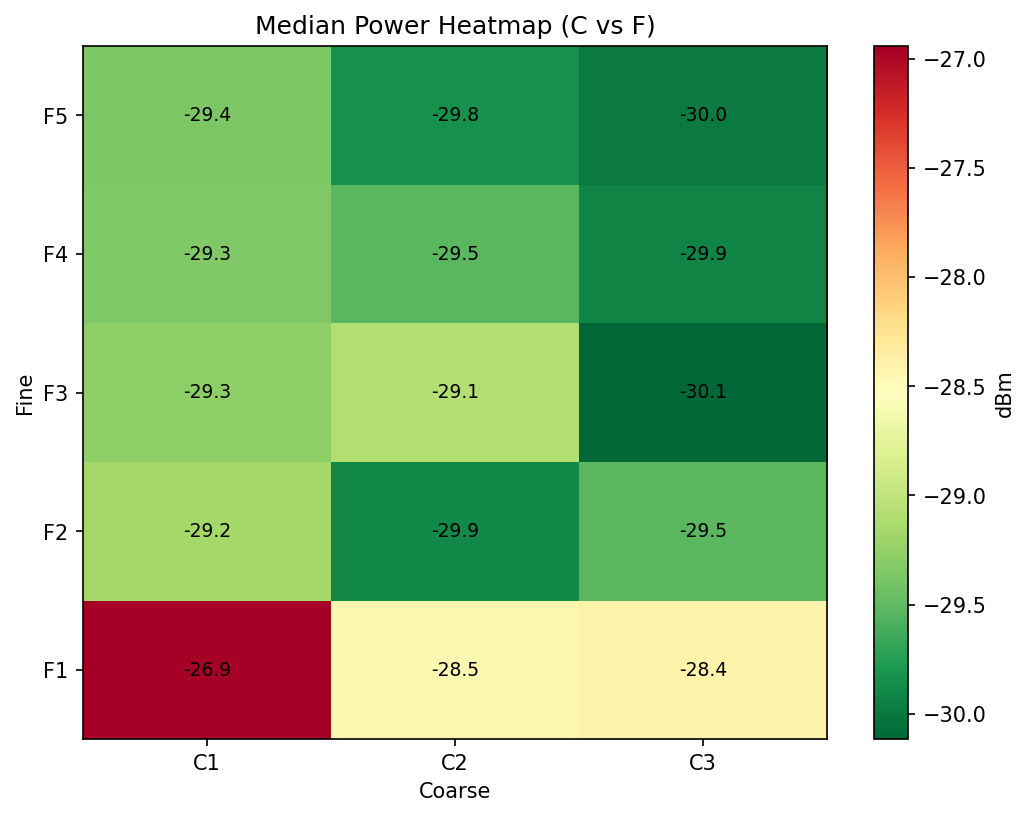
\includegraphics[width=0.48\textwidth]{figures/heatmap_power_median.png}
    \caption{Heatmap of median achieved power for all C1--C3 configurations. Lower (more negative, darker green) is better.}
    \label{fig:heatmap_power}
\end{figure}

\begin{figure}[htbp]
    \centering
    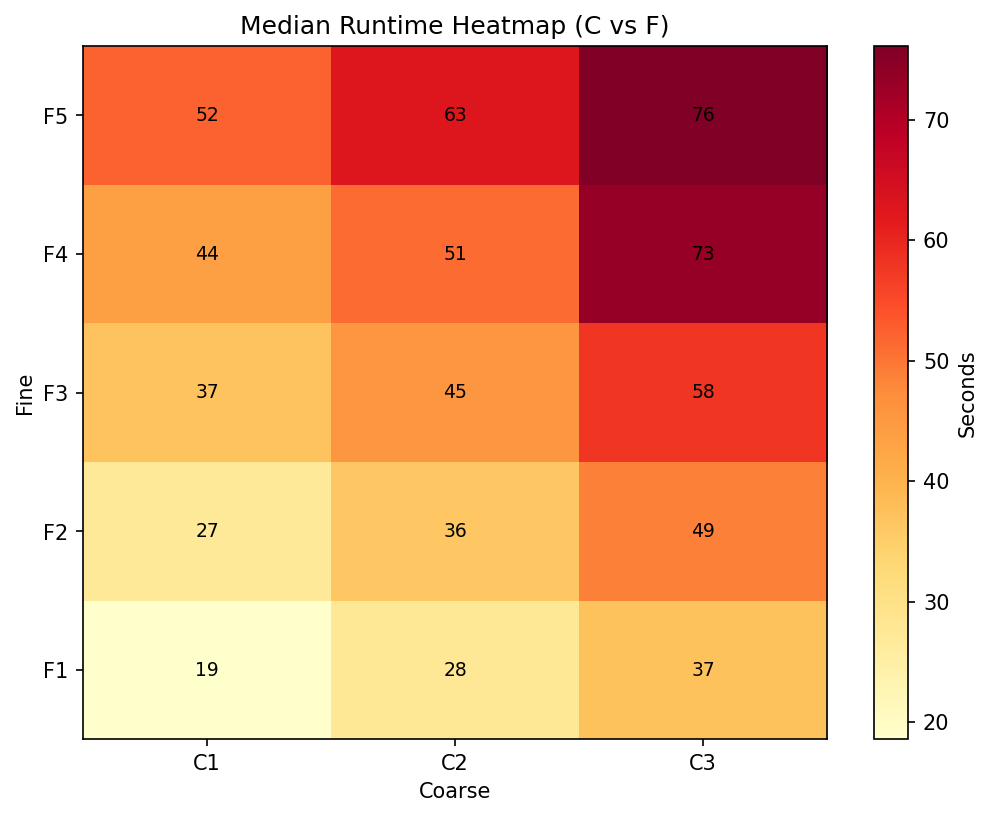
\includegraphics[width=0.48\textwidth]{figures/heatmap_runtime_median.png}
    \caption{Heatmap of median runtime for all C1--C3 configurations. Lower (lighter colour) is faster.}
    \label{fig:heatmap_runtime}
\end{figure}

Figure~\ref{fig:power_lines} and Figure~\ref{fig:runtime_lines} show the mean power and mean runtime as a function of iteration count. Increasing the number of fine iterations yields diminishing improvements in power: from F1 to F2 the mean improvement is approximately 1.5\,dB across all coarse levels, whereas from F3 to F5 the improvement is less than 0.5\,dB. Each additional coarse iteration adds roughly 10--15\,s to the mean runtime and improves the mean power by 0.3--0.8\,dB.

\begin{figure}[htbp]
    \centering
    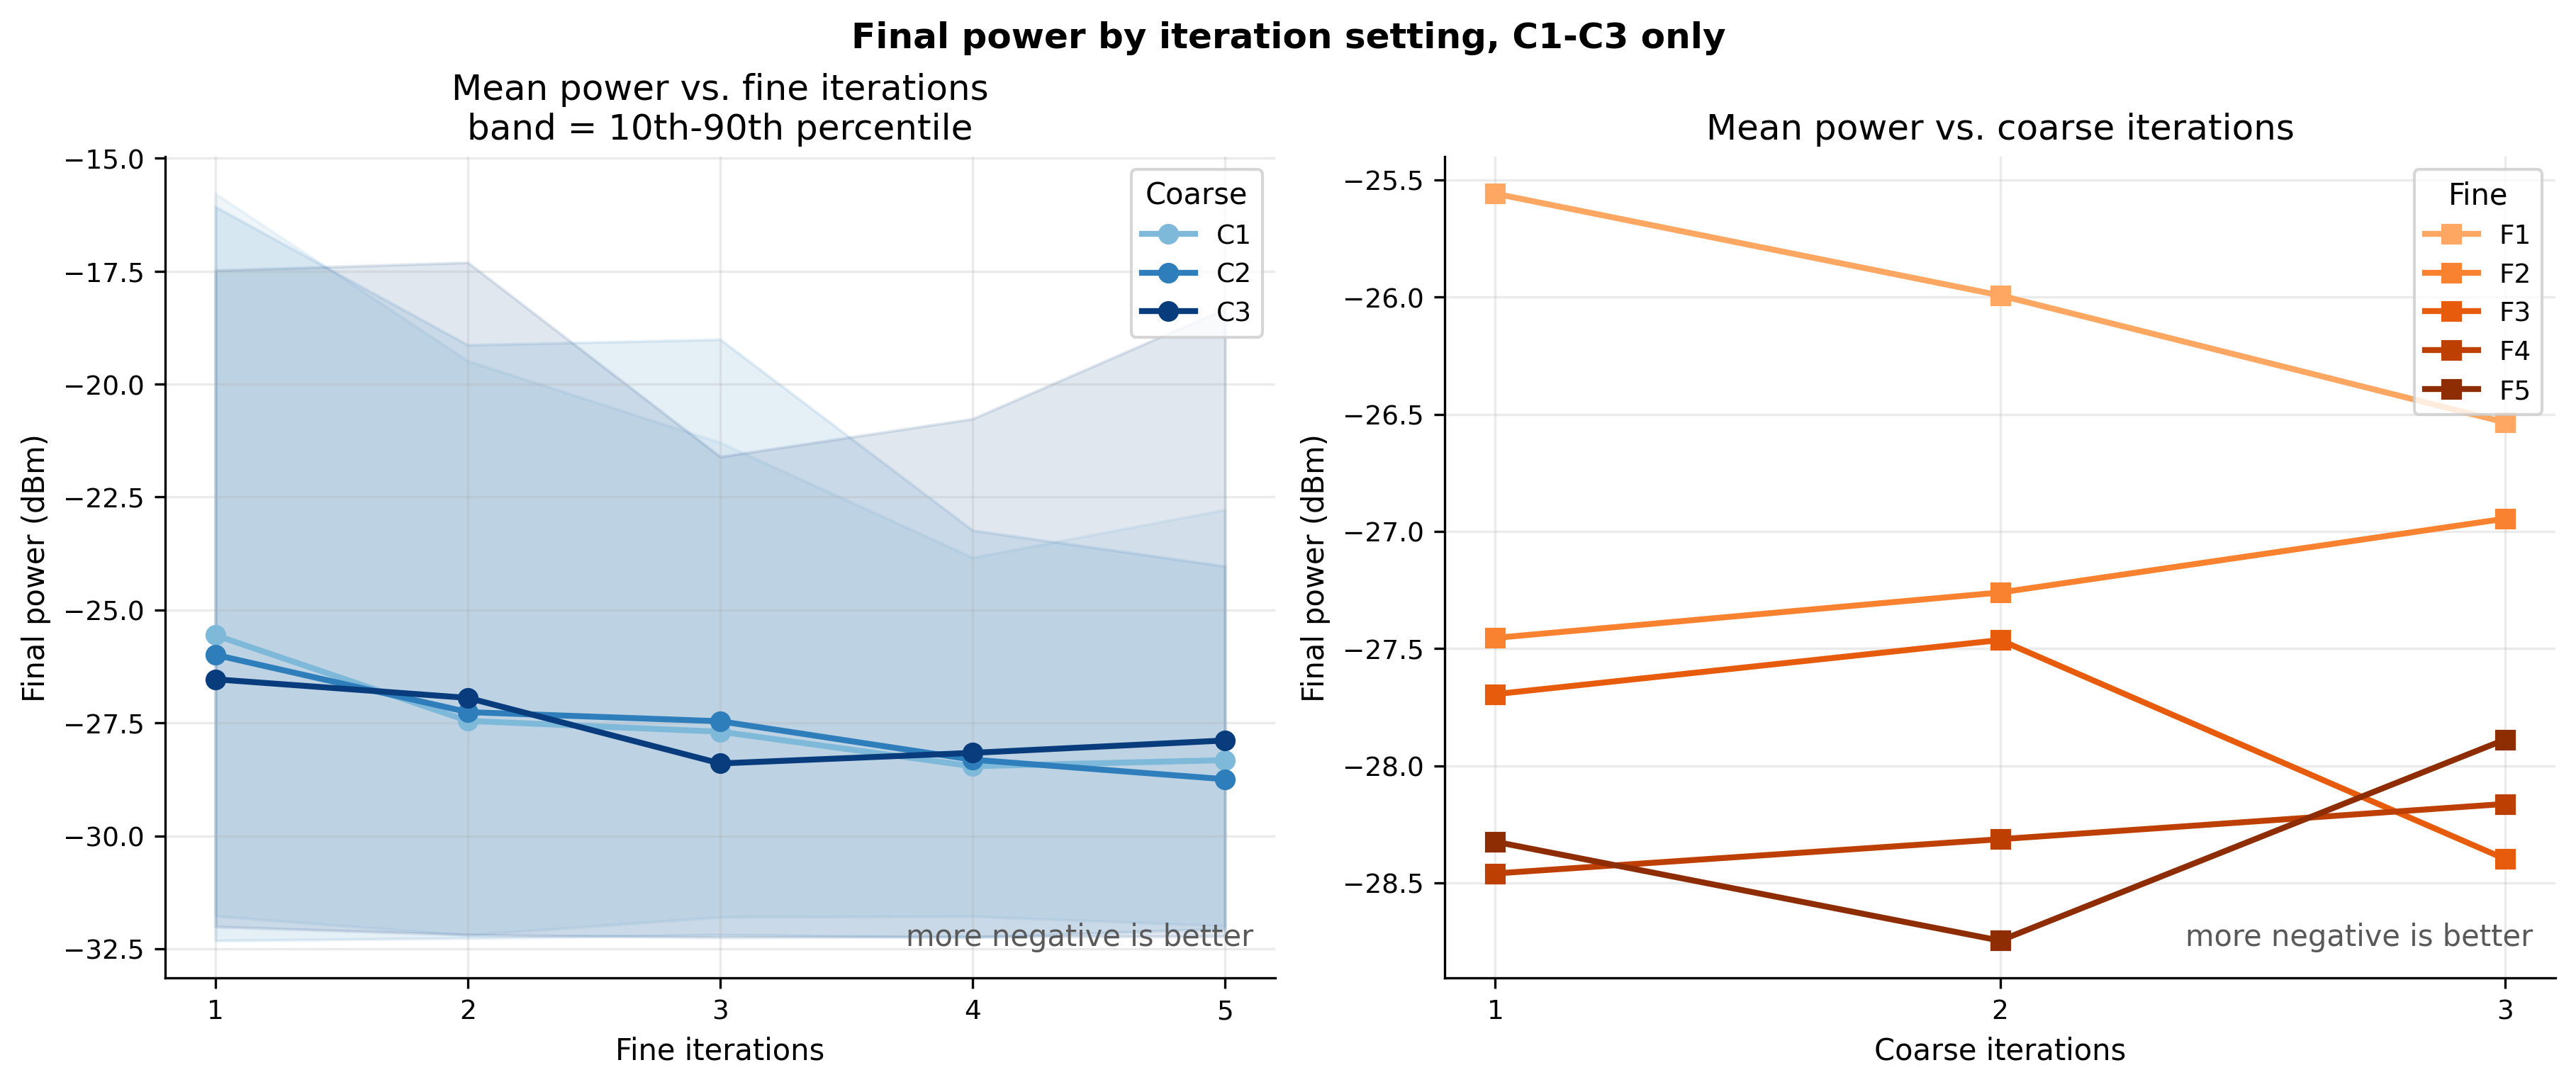
\includegraphics[width=0.7\textwidth]{figures/power_lines_c1_c3.png}
    \caption{Mean power as a function of fine iterations (left) and coarse iterations (right), with 10th--90th percentile bands. More negative is better.}
    \label{fig:power_lines}
\end{figure}

\begin{figure}[htbp]
    \centering
    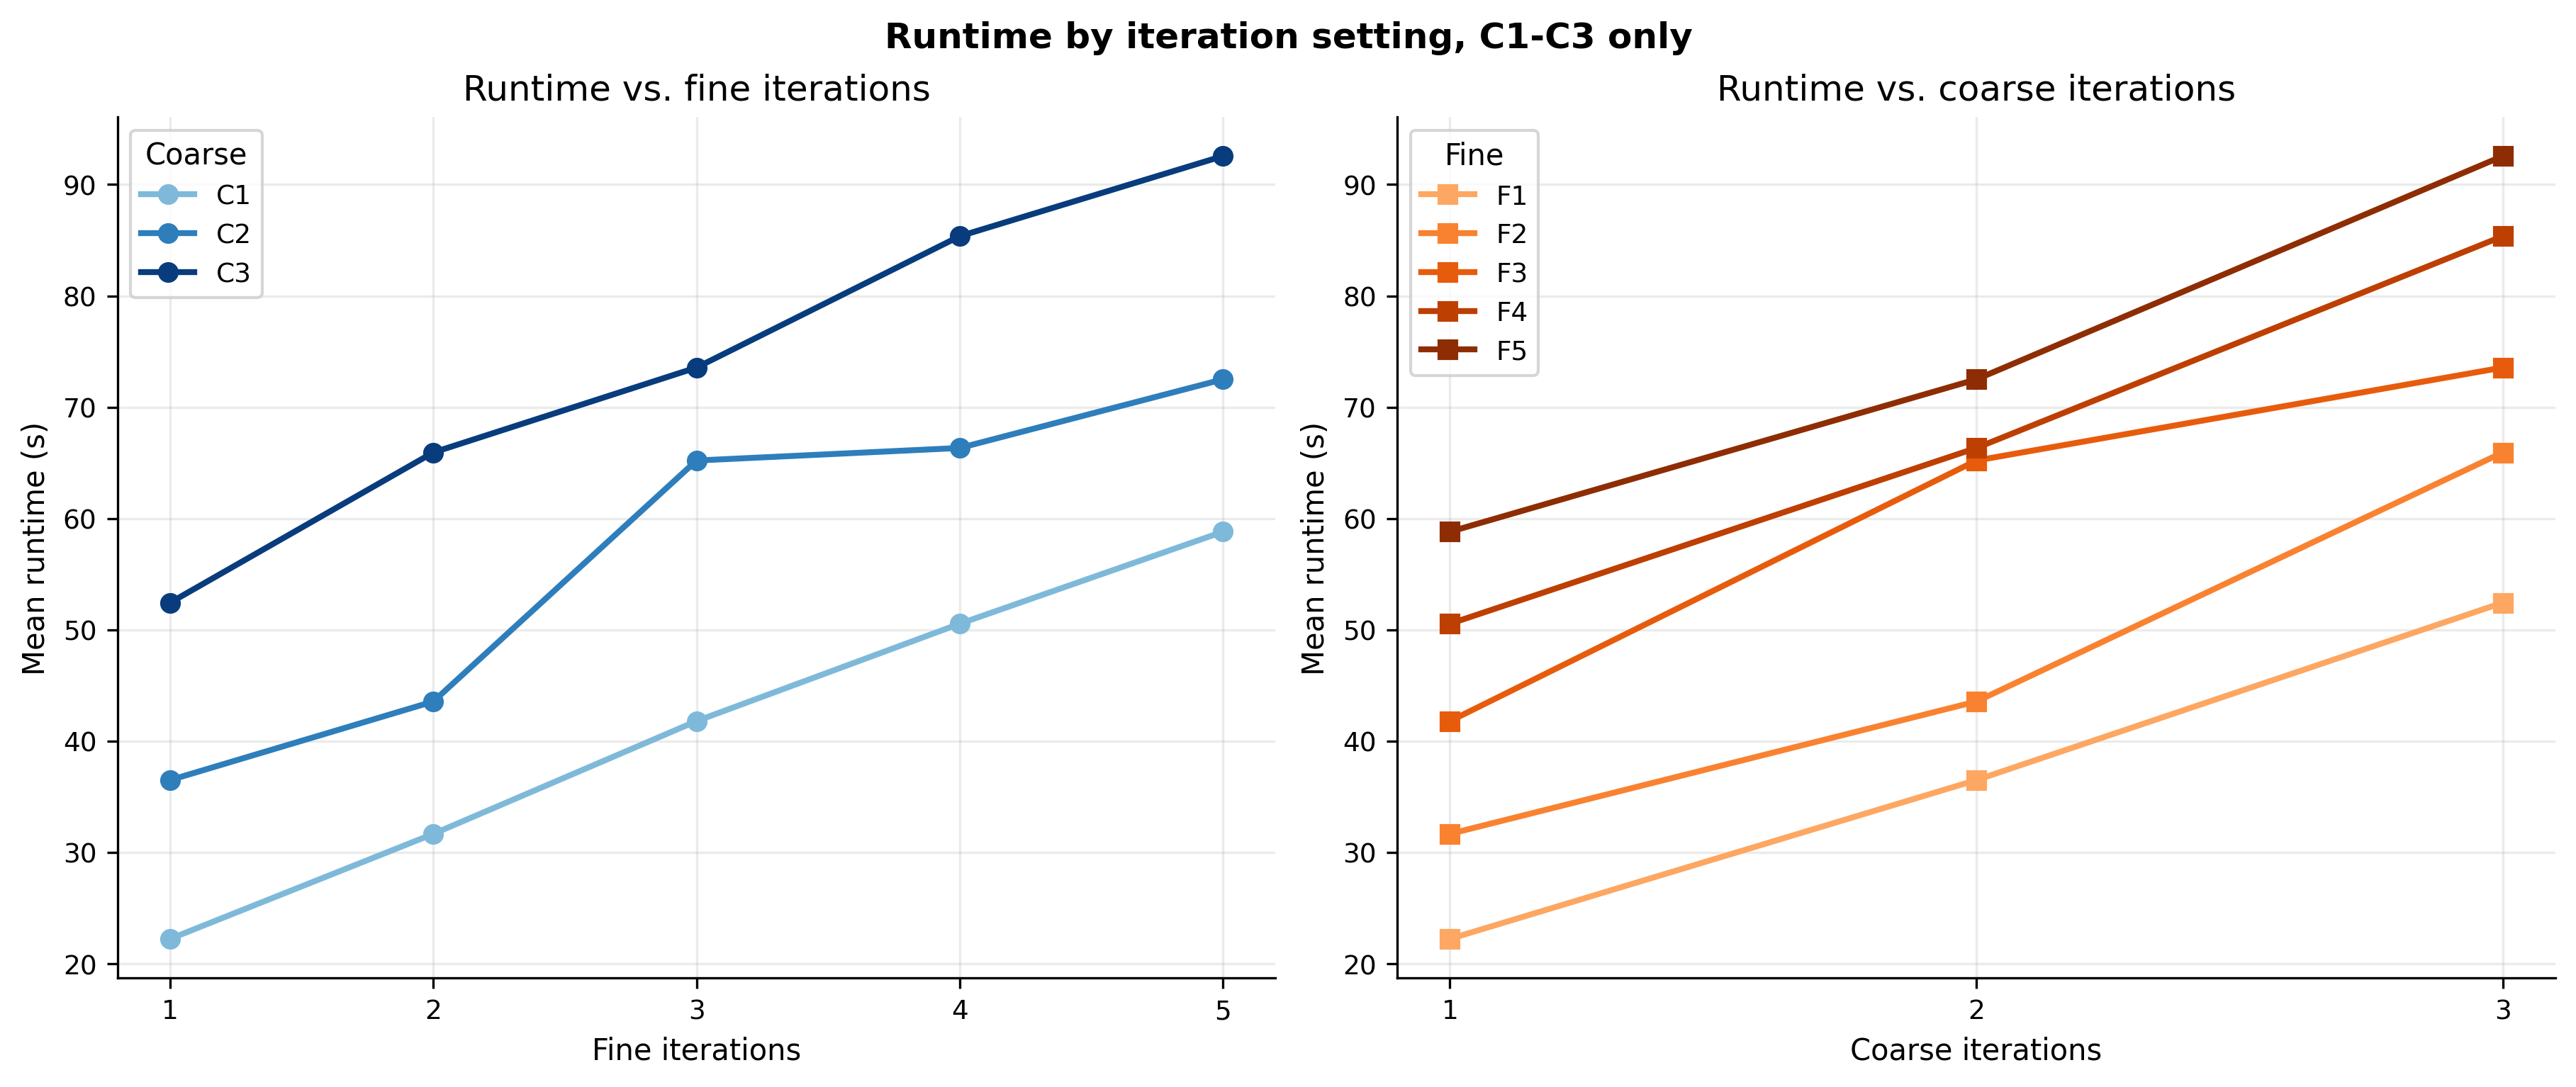
\includegraphics[width=0.7\textwidth]{figures/runtime_lines_c1_c3.png}
    \caption{Mean runtime as a function of fine iterations (left) and coarse iterations (right).}
    \label{fig:runtime_lines}
\end{figure}

C2F2 achieved a median of $-29.9$\,dBm at a median runtime of 36\,s with 49\,\% of runs below $-30$\,dBm. C3F3 reached the best median power ($-30.1$\,dBm) with 53\,\% below $-30$\,dBm, but at a median runtime of 58\,s. The best single-run power across all configurations was $-34.2$\,dBm (C1F5).

\subsection{Paddle order: HQQ vs.\ QHQ}
\label{sec:arm_order}

Two paddle optimization orders were compared over 496 runs using the C2F2 configuration, alternating between HQQ and QHQ. Table~\ref{tab:arm_order} summarizes the results.

\begin{table}[htbp]
    \centering
    \caption{Comparison of paddle orders over 496 optimizations (C2F2 configuration). Power in dBm.}
    \label{tab:arm_order}
    \begin{tabular}{l r r r r r}
        \hline
        Order & Count & Mean & Median & Std & Min \\
        \hline
        HQQ & 247 & $-28.4$\,dBm & $-29.1$\,dBm & 3.0\,dBm & $-33.3$\,dBm \\
        QHQ & 249 & $-27.4$\,dBm & $-27.9$\,dBm & 3.1\,dBm & $-32.8$\,dBm \\
        \hline
    \end{tabular}
\end{table}

HQQ achieved 1.0\,dB lower mean power and 1.2\,dB lower median power than QHQ, with comparable standard deviation (3.0 vs.\ 3.1\,dBm). Figure~\ref{fig:arm_order_boxplot} shows the distributions.

\begin{figure}[htbp]
    \centering
    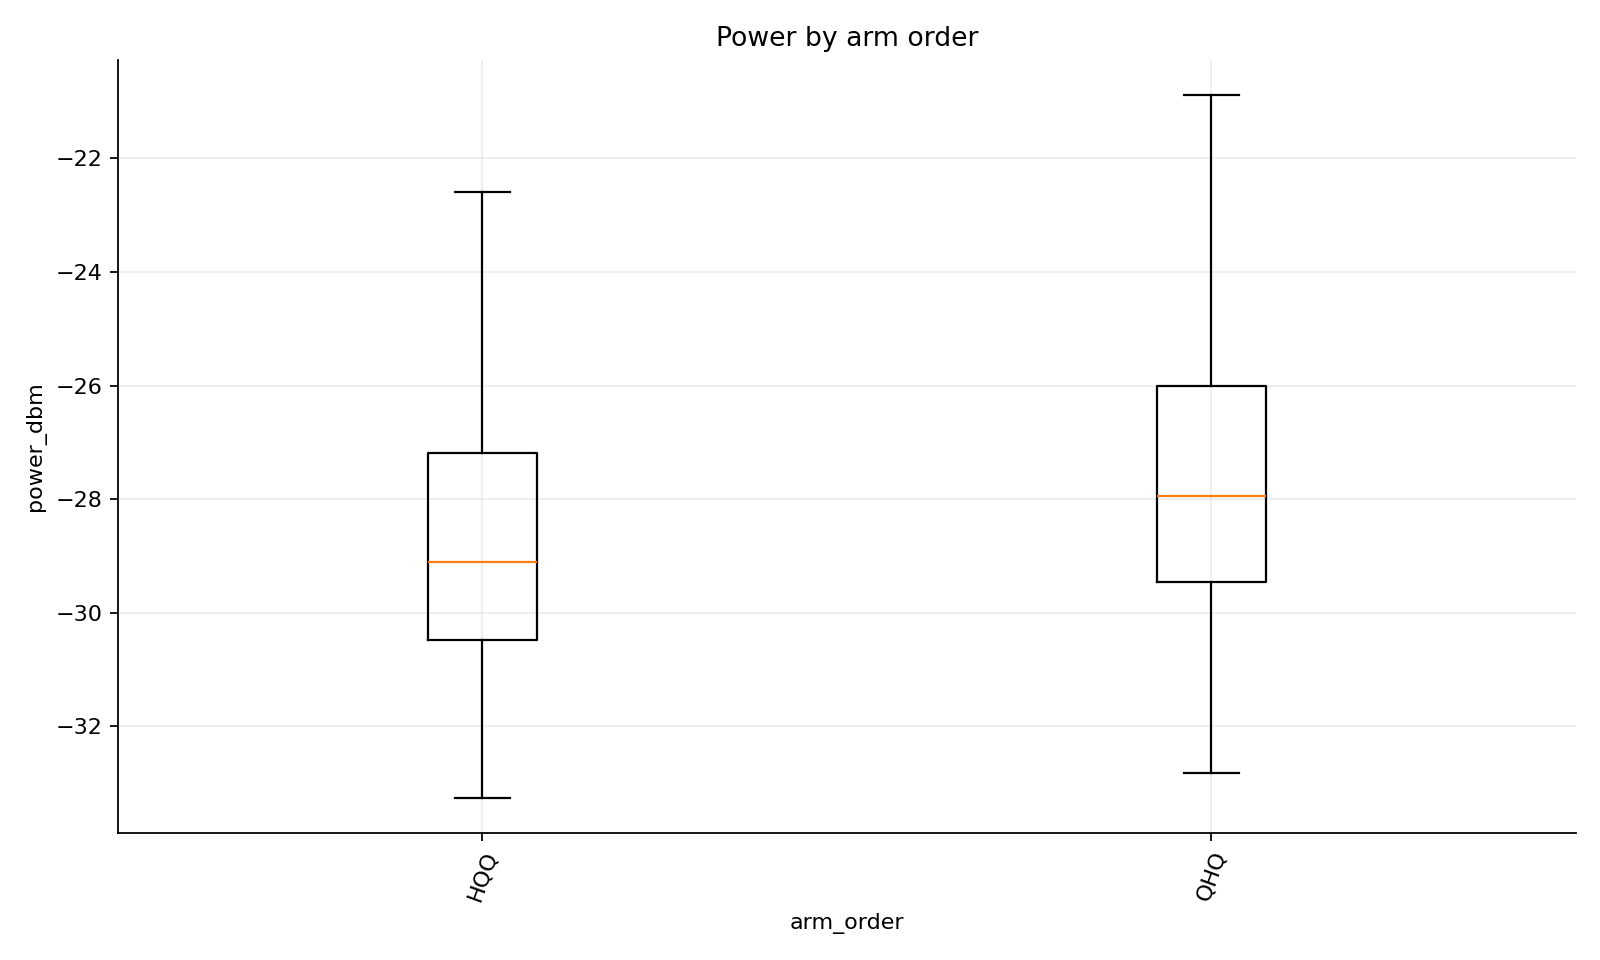
\includegraphics[width=0.5\textwidth]{figures/arm_order_boxplot_new.png}
    \caption{Box plot of achieved power by paddle order (HQQ vs.\ QHQ). HQQ shows a lower (better) median and tighter interquartile range.}
    \label{fig:arm_order_boxplot}
\end{figure}

\subsection{Long-term stability and drift}
\label{sec:drift}

The system was run continuously for 66.6 hours (June~12 at 14:38 to June~15 at 09:15), logging the optical power every 61\,s between optimizations. A total of 3{,}913 drift samples and 75 automatic optimizations were recorded. Table~\ref{tab:drift_summary} summarizes the drift measurements.

\begin{table}[htbp]
    \centering
    \caption{Summary statistics for drift measurements over 66.6 hours (3{,}913 samples).}
    \label{tab:drift_summary}
    \begin{tabular}{l r}
        \hline
        Metric & Value \\
        \hline
        Duration                   & 66.6\,h \\
        Drift samples              & 3{,}913 \\
        Automatic optimizations    & 75 \\
        Mean drift power           & $-24.3$\,dBm \\
        Median drift power         & $-23.9$\,dBm \\
        Standard deviation         & 3.3\,dBm \\
        Best sample                & $-34.1$\,dBm \\
        Worst sample               & $-6.9$\,dBm \\
        Fraction below $-20$\,dBm & 98.1\,\% \\
        \hline
    \end{tabular}
\end{table}

Figure~\ref{fig:day_night} shows the power behaviour over the full measurement period. The upper panel displays the time series with a 20-minute rolling median; the lower panel folds the data into a typical daily pattern. A clear diurnal variation is visible: the nighttime standard deviation (00:00--06:00) was 1.9\,dBm, compared to 3.4\,dBm during daytime hours (06:00--18:00). The worst individual measurement ($-6.9$\,dBm) occurred during the afternoon (hour~14), and a second outlier of $-7.3$\,dBm appeared at hour~9.

\begin{figure}[htbp]
    \centering
    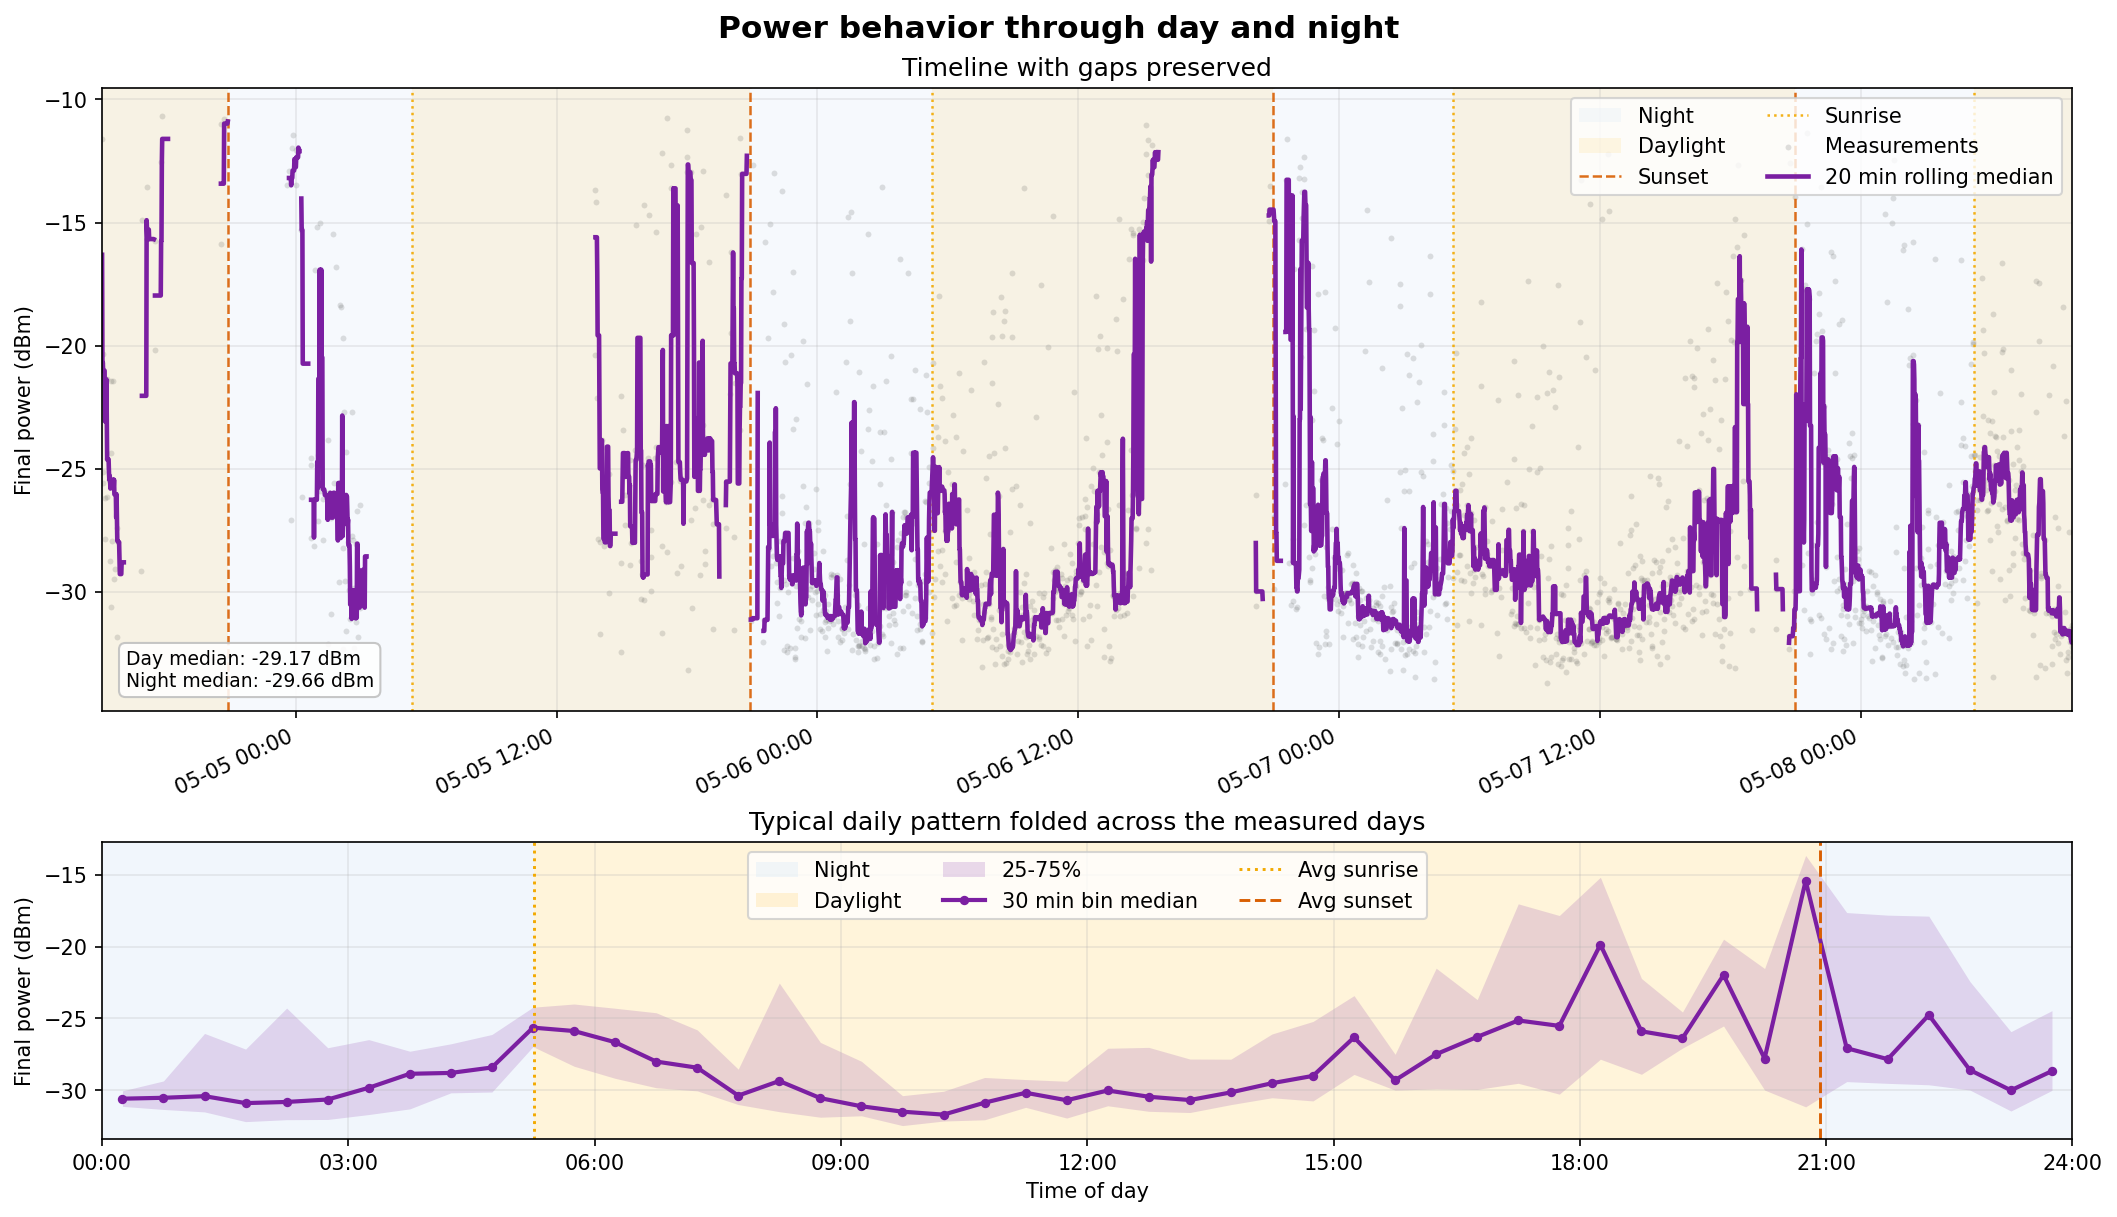
\includegraphics[width=\textwidth]{figures/day_night_power.png}
    \caption{Power behaviour through day and night. Upper: full time series with rolling median and day/night shading. Lower: daily pattern folded across the measured days, with 30-minute bin medians and 25th--75th percentile band. Day median: $-29.2$\,dBm; night median: $-29.7$\,dBm.}
    \label{fig:day_night}
\end{figure}

Between consecutive drift samples (median interval 61\,s), the median power change was 0.10\,dB and the standard deviation was 1.14\,dB. The largest observed step change was 21.1\,dB.

Figure~\ref{fig:survival} shows the survival curve: the probability that the power remains below $-20$\,dBm for at least $T$ consecutive minutes. After a successful optimization, there is an 81\,\% probability that the power stays below $-20$\,dBm for at least 10 minutes, a 60\,\% probability for 30 minutes, and a 22\,\% probability for 60 minutes.

\begin{figure}[htbp]
    \centering
    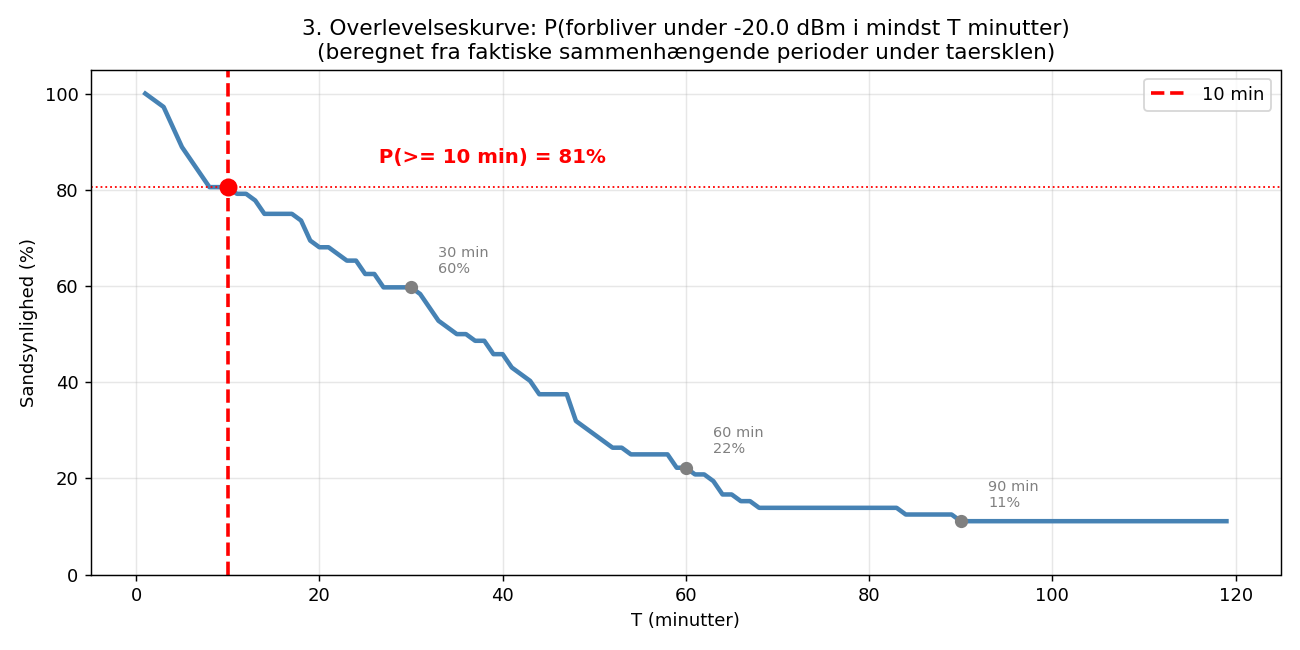
\includegraphics[width=0.7\textwidth]{figures/survival_curve.png}
    \caption{Survival curve: probability that the power remains below $-20$\,dBm for at least $T$ consecutive minutes.}
    \label{fig:survival}
\end{figure}

\subsection{Automated vs.\ manual runtime}

A manual optimization of the polarization controller typically takes several minutes per attempt, depending on operator experience. The automated system completed each optimization in a median of 34\,s (mean 36.8\,s). Over the 66.6-hour test period, the system performed 75 optimizations without human intervention.
